\documentclass{article}

%%%%%%%%%%%%%%%%%%%%%%%%%%%%%%%%%%%%%%%%
%% Packages
%%%%%%%%%%%%%%%%%%%%%%%%%%%%%%%%%%%%%%%%

\usepackage[english]{babel}

% Margins
\usepackage[margin=1in]{geometry}
% Spaced paragraphs
\usepackage[parfill]{parskip}
% Fancy headers
\usepackage{fancyhdr}
% Allow use of titles
\usepackage{titling}

% Maths stuff
\usepackage{amsmath}
\usepackage{amsfonts}
\usepackage{amssymb}
\usepackage{amsthm}
\usepackage{physics}
\usepackage{bm}
\usepackage{turnstile}

% Links
\usepackage[hidelinks]{hyperref}

% Allow repetition in macros
\usepackage{multido}

% Set up theorem and definition environments
\newtheorem{theorem}{Theorem}
\newtheorem{definition}{Definition}

%%%%%%%%%%%%%%%%%%%%%%%%%%%%%%%%%%%%%%%%
%% Tikz
%%%%%%%%%%%%%%%%%%%%%%%%%%%%%%%%%%%%%%%%

%\usepackage{subcaption}
\usepackage{tikz}
\usetikzlibrary{automata}
\usetikzlibrary{arrows}
\usetikzlibrary{arrows.meta}
\usetikzlibrary{calc}

\tikzset{
	%	vertex/.style={circle,draw,minimum size=1.5em},
	%	main node/.style={circle,draw,font=\sffamily\Large\bfseries},
	%	main node/.style={circle,thick,draw},
	edge/.style={->,> = latex'}
}

%%%%%%%%%%%%%%%%%%%%%%%%%%%%%%%%%%%%%%%%
%% Set Theory Macros
%%%%%%%%%%%%%%%%%%%%%%%%%%%%%%%%%%%%%%%%

% Naturals
\newcommand{\Nat}{\mathbb{N}}
% Integers
\newcommand{\Int}{\mathbb{Z}}
% Rationals
\newcommand{\Rationals}{\mathbb{Q}}
% Reals
\newcommand{\Reals}{\mathbb{R}}

% Use small arrows for implies / iff
\renewcommand{\implies}{\rightarrow}
\renewcommand{\iff}{\leftrightarrow}

% Use bold for vectors
\renewcommand{\vec}[1]{\mathbf{#1}}

% Notation for a set (easier than \lbrace \rbrace :P)
\newcommand{\set}[1]{\left\lbrace #1 \right\rbrace}

% Notation for a set comprehension / set builder notation
\newcommand{\setcomp}[2]{\set{#1 \, | \, #2}}

% Notation for a set comprehension with two conditions
\newcommand{\setcompdouble}[3]{\set{#1 \, | \, #2 \, | \, #3}}

% Notation for a tuple
\newcommand{\tuple}[1]{\left\langle #1 \right\rangle}

% Notation for a pair
\newcommand{\pair}[2]{\tuple{#1, #2}}

% Powerset
\newcommand{\powerset}[1]{\mathcal{P}(#1)}

% Ordinals
\newcommand{\On}{\bm{On}}
% Language
\newcommand{\Lang}{\mathcal{L}}
% Language of Set Theory
\newcommand{\LangSet}{\Lang_\in}

% Model
\newcommand{\Model}{\mathcal{M}}

% Function notation for injection / surjection / bijection
\newcommand{\surject}{\twoheadrightarrow}
\newcommand{\inject}{\rightarrowtail}
\newcommand{\biject}{\mathbin{\rightarrowtail \hspace{-8pt} \twoheadrightarrow}}

% Russell's set
\newcommand{\RussellSet}{\setcomp{z \in x}{z \notin z}}

%%%%%%%%%%%%%%%%%%%%%%%%%%%%%%%%%%%%%%%%
%% Computability Theory Macros
%%%%%%%%%%%%%%%%%%%%%%%%%%%%%%%%%%%%%%%%

% Turing machine computes
\newcommand{\turingcomputes}[1]{\xrightarrow[#1]{}}

% Class

\newcommand{\Class}{\mathcal{C}}

% Projection function
\newcommand{\proj}[2]{\pi_{#1, #2}}

% Proper subtraction / 'monus'
\providecommand{\monus}{% Don't redefine it if available
	\mathbin{% We want a binary operation
		\vphantom{+}% The same height as a plus or minus
		\text{% Change size in sub/superscripts
			\mathsurround=0pt % To be on the safe side
			\ooalign{% Superimpose the two symbols
				\noalign{\kern-.35ex}% but the dot is raised a bit
				\hidewidth$\smash{\cdot}$\hidewidth\cr % Dot
				\noalign{\kern.35ex}% Backup for vertical alignment
				$-$\cr % Minus
			}%
		}%
	}%
}

%%%%%%%%%%%%%%%%%%%%%%%%%%%%%%%%%%%%%%%%
%% Titles
%%%%%%%%%%%%%%%%%%%%%%%%%%%%%%%%%%%%%%%%

\title{MATH3306 Course Notes -- \url{https://github.com/mcoot/CourseNotes} }
\author{Joseph Spearritt}

\pagestyle{fancy}
\lhead{\thetitle}
\rhead{\theauthor}
\cfoot{\thepage}

\begin{document}
	\section{Finite State Automata}

\subsection{Alphabets \& Strings}

\begin{itemize}
	
	\item Let $ A $ be a set; then $ A^n $ is the set of all finite sequences $ a_1 \dots a_n $ with $ a_i \in A $, $ 1 \le i \le m $
	
	\begin{itemize}
		\item Elements of $ A $ are \textit{letters} or \textit{symbols}
		
		\item Elements of $ A^n $ are \textit{words} or \textit{strings} over $ A $ of length $ m $
	\end{itemize}

	\item $ \varepsilon $ is the special \textit{empty string}, the only string of length $ 0 $

	\item $ A^+ = \bigcup_{m \ge 1} A^m $ -- the set of non-empty strings over $ A $ of any length
	
	\item $ A^* = A^+ \cup \varepsilon = \bigcup_{m \ge 0} A^m$ -- the set of (possibly empty) strings over $ A $ of any length
	
	\item If $ \alpha = a_1 \dots a_m $, $ \beta = b_1 \dots b_m \in A^* $, then define $ \alpha \beta $ to be $ a_1 \dots a_m b_1 \dots b_m \in A^{m + n} $. This gives binary `product' or \textit{concatenation} on $ A^* $
	
	\item For $ \alpha \in A^+ $, define $ \alpha^n, n \in \Nat $ by $ \alpha^0 = \varepsilon $, and $ \alpha^{n+1} = \alpha^n \alpha $
	
	\item A \textit{language} with alphabet $ A $ is a subset of $ A^* $
	
\end{itemize}

\clearpage

\subsection{Definition of an FSA}

\begin{itemize}
	
	\item A Finite State Automaton (FSA) is a tuple $ M = (Q, F, A, \tau, q_0) $
	
	\begin{itemize}
		
		\item $ Q $ is a finite set of states
		
		\item $ F \subseteq Q $ is the set of final states
		
		\item $ A $ is the alphabet
		
		\item $ \tau \subseteq Q \times A \times Q $ is the set of transitions
		
		\item $ q_0 \in Q $ is the initial state
		
	\end{itemize}

	\item The transition diagram of an FSA is a directed graph with:
	
	\begin{itemize}
		
		\item Vertex set $ Q $
		
		\item An edge for each transition; $ (q, a, q') \in \tau $ corresponds to an edge from $ q $ to $ q' $ with label $ a $
		
		\item Initial state $ q_0 $ labelled with $ - $
		
		\item Final states labelled with $ + $
		
		\item Example: a \textit{non-deterministic} `haha machine', with $ A = \set{h, a} $
		
		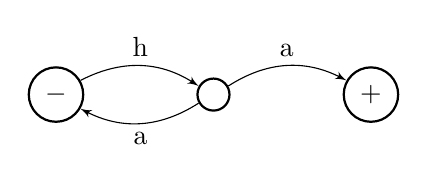
\begin{tikzpicture}
		\node[circle,thick,draw] (q0) at (0, 0) {$ - $};
		\node[circle,thick,draw] (q1) at (2, 0) {$ \; $};
		\node[circle,thick,draw] (q2) at (4, 0) {$ + $};
		
		\draw[edge] (q0) to[bend left] node[above] {h} (q1);
		\draw[edge] (q1) to[bend left] node[above] {a} (q2);
		\draw[edge] (q1) to[bend left] node[below] {a} (q0);
		\end{tikzpicture}
		
	\end{itemize}

	\item A \textit{computation} of $ M $ is a sequence $ q_0, a_1, q_1, a_2, \dots, a_n, q_n $ with $ n \ge 0 $ where $ (q_i, a_{i+1}, q_{i+1}) \in \tau $ for $ 0 \le i \le n - 1 $
	
	\begin{itemize}
		
		\item The \textit{label} on the computation is $ a_1 \dots a_m $
		
		\item The computation is \textit{successful} if $ q_n \in F $
		
		\item A string $ a_1 \dots a_n $ is \textit{accepted} by $ M $ if there is a successful computation with label $ a_1 \dots a_n $, and it is \textit{rejected} otherwise
		
	\end{itemize}

	\item The language recognised by $ M $ is $ \Lang(M) = \setcomp{w \in A^*}{w \text{ is accepted by } M} $
	
	\item There is a one-to-one correspondence between computations of $ M $ and paths in the graph from $ q_0 $	
	
	\item Example: $ A = \set{a, b} $ of an FSA accepting only words with an odd number of 'a's
	
	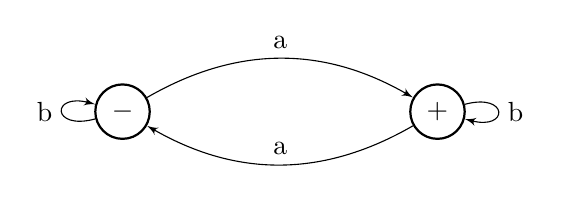
\begin{tikzpicture}
	\node[circle,thick,draw] (q0) at (0, 0) {$ - $};
	\node[circle,thick,draw] (q1) at (4, 0) {$ + $};
	
	\draw[edge] (q0) to[bend left] node[above] {a} (q1);
	\draw[edge] (q0) to[loop left] node[left] {b} (q0);
	
	\draw[edge] (q1) to[bend left] node[above] {a} (q0);
	\draw[edge] (q1) to[loop right] node[right] {b} (q1);
	\end{tikzpicture}
	
	\item An FSA is deterministic (a DFA) if for all $ q \in Q, a \in A $ there is exactly one $ q' \in Q $ such that $ (q, a, q') \in \tau $
	
	\item Example: DFA for the `haha machine'
	
	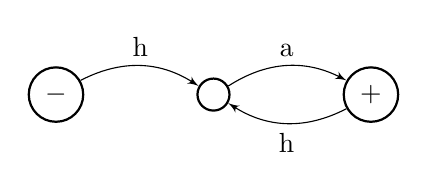
\begin{tikzpicture}
	\node[circle,thick,draw] (q0) at (0, 0) {$ - $};
	\node[circle,thick,draw] (q1) at (2, 0) {$ \; $};
	\node[circle,thick,draw] (q2) at (4, 0) {$ + $};
	
	\draw[edge] (q0) to[bend left] node[above] {h} (q1);
	\draw[edge] (q1) to[bend left] node[above] {a} (q2);
	\draw[edge] (q2) to[bend left] node[below] {h} (q1);
	\end{tikzpicture}
	
	\item Note this machine lacks a transition for $ a $ when in the initial state -- though technically required for a DFA, it is easily fixed by adding an `error state' to catch what would otherwise be missing transitions
	
\end{itemize}

\clearpage

\subsection{Deterministic FSAs}

\begin{itemize}
	
	\item For a DFA $ M $, define the transition function $ \delta: Q \times A \to Q $ by $ q' = \delta(q, a) $, where $ q' $ is the unique element such that $ (q, a, q') \in \tau $
	
	\item If $ \Lang $ is a language with alphabet $ A $, then the following are equivalent:
	
	\begin{enumerate}
		\item $ \Lang $ is recognised by an FSA
		
		\item $ \Lang $ is recognised by a DFA
	\end{enumerate}
	
	\item Given a non-deterministic FSA $ M = (Q, F, A, \tau, q_0) $, an equivalent DFA $ M' = (Q', F', A, \tau', q_0') $ may be generated by the \textit{powerset method}:
	
	\begin{itemize}
		
		\item $ Q' = \powerset{Q} \setminus \emptyset $ (i.e. the set of all subsets of $ Q $ that aren't empty)
		
		\item $ F' = \setcomp{X \in Q'}{q \in X \text{ for some } q \in F} $
		
		\item For $ X \in Q', a \in A $, define $ \delta(X, a) := \setcomp{q \in Q}{(x, a, q) \in \tau \text{ for some } x \in X} $
		
		\item $ \tau' = \setcomp{(X, a, \delta(X, a))}{X \in Q', a \in A} $
		
		\item $ q_0' = \set{q_0} $
		
	\end{itemize}

	\item Proof: show that $ \Lang(M) = \Lang(M') $
	
	\begin{itemize}
		\item $ \Lang(M) \subseteq Lang(M') $:
		
		\begin{itemize}
			\item Given $ w \in \Lang(M) $, $  q_0 a_1 \dots a_n q_n $ is a successful computation of $ M $
			
			\item Then define $ q_i' = \delta(q_{i-1}', a_i) $ for $ 1 \le i \le n $
			
			\item $ q_0', a_1, q_1' \dots a_n, q_n' $ will be a successful computation of $ M' $
			
			\item Therefore $ w \in \Lang(M') $
		\end{itemize}
	
	\item $ \Lang(M') \subseteq Lang(M) $:
	
	\begin{itemize}
		\item Let $ w = a_1 \dots a_n \in L(M') $, and $  q_0', a_1, q_1' \dots a_n, q_n' $ be a successful computation of $ M $
		
		\item Each $ q_i' $ cannot be the empty set
		
		\item By definition of $ \tau' $, $ \exists q_1 \in q_1' $ s.t. $ (q_0, a_1, q_1) \in \tau $
		
		\item Then we can find $ q_i \in q_i' $ s.t. $ (q_{i-1}, a_i, q_i) \in \tau $ for $ 1 \le i \le n $
		
		\item For $ q_n $ we further require $ q_n \in F $
		
		\item Therefore, $ q_0, a_1, q_1, a_2, \dots a_n, q_n $ is a successful computation
		
		\item Therefore $ w \in \Lang(M) $
	\end{itemize}
	
	\end{itemize}
	
\end{itemize}

\clearpage

\subsection{The Pumping Lemma}

\begin{itemize}
	
	\item The Pumping Lemma says that for any $ \Lang $ recognised by an FSA $ M $, there is a certain word length beyond which all words can be split into sections as $ xyz$, where $ x y^n z $ is also in the language
	
	\item Formally there is an integer $ p > 0 $ s.t. any word $ w \in L $ with $ \abs{w} \ge p $ is of the form $ w = xyz $, where $ \abs{y} > 0 $, $ \abs{xy} \le p $ and $ x y^i z \in \Lang $ for $ i \ge 0 $
	
	\item Proof:
	
	\begin{itemize}
		
		\item Let $ p $ be the number of states in $ M $, and suppose $ w = a_1 \dots a_n \in \Lang $, where $ n \ge p $
		
		\item A successful computation $ q_0, a_1, \dots, q_n $ has to pass through a certain state at least twice (by the pigeonhole principle)
		
		\item Therefore, $ \exists r < s $ s.t. $ q_r = q_s $; choose minimal such $ s $
		
		\item Now put $ x = a_1 \dots a_r $, $ y = a_{r+1} \dots a_s $ (note $ \abs{y} > 0$), and $ z = a_{s+1} \dots a_n $
		
		\item By minimality of $ s $, $ q_0, \dots q_{s-1} $ are distinct, and $ \abs{xy} = s \le p $
		
		\item Then, note that $ q_r, a_{r+1}, \dots, q_{s} $ is a loop, which may be validly repeated $ i \ge 0 $ times
		
		\item Therefore, $ x y^i z \in \Lang $
		
	\end{itemize}

	\item Corollary: there exist languages which are not computable by an FSA
	
	\item Example: there is no FSA which can recognise $ \Lang = \setcomp{a^n b^n}{n \in \Nat} $
	
	\item Proof:
	
	\begin{itemize}
		
		\item Assume for a contradiction there exists an FSA $ M $ which can recognise $ \Lang $
		
		\item Let $ p $ be the number from the pumping lemma, and choose $ n \ge p $ and consider $ w = a^n b^n $

		\item By the pumping lemma, $ \exists x, y, z $ s.t. $ a^n b^n = xyz $, with $ \abs{y} \ge 1 $ and $ \abs{xy} \le p \le n $
		
		\item Then $ y $ is written entirely in terms of the letter a, and $ \abs{y} \ge 1 $
		
		\item By the pumping lemma, $ x y^i z \in \Lang $ for all $ i $
		
		\item So choose $ i = 0 $, then some $ w = a^k b^n \in \Lang $ s.t. $ k < n $, which is a contradiction 
		
	\end{itemize}
	
\end{itemize}

	\section{Turing Machines}

\subsection{Definition}

\begin{itemize}
	
	\item A Turing machine is a tuple $ T = (Q, F, A, I, \tau, q_0) $
	
	\begin{itemize}
		
		\item $ Q $ is a finite set of states
		
		\item $ F \subseteq Q $ is the set of final states
		
		\item $ A $ is a finite set, the tape alphabet, with a distinguished blank symbol $ B \in A $
		
		\item $ I $ is a subset of $ A \setminus \set{B} $, the input alphabet
		
		\item $ \tau \subseteq Q \times A \times Q \times A \times \set{L, R} $ is the set of transitions
		
		\item $ q_0 \in Q $ is the initial state
				
	\end{itemize}
	
	\item As in an FSA, non-determinism is allowed
	
	\item The tape is infinite in both directions, but only ever contains a finite number of non-blank symbols
	
	\item A \textit{tape description} for $ T $ is a triple $ (a, \alpha, \beta) $ with $ a \in A $, and $ \alpha: \Nat \to A $ and $ \beta: \Nat \to A $ being functions with $ a(n) = B $ and $ B(n) = B $ for all but finitely many $ n \in \Nat $
	
	\begin{itemize}
		\item So the tape looks like: $ \dots BBB \beta(l) \beta(l - 1) \dots \beta(0) \underline{a} \alpha(0) \alpha(1) \dots \alpha(r) BBB \dots $, with $ l, r \in \Nat $
	\end{itemize}
	
	\item A \textit{configuration} of $ T $ is a tuple $ (q, a, \alpha, \beta) $ where $ q \in Q $ and $ (a, \alpha, \beta) $ is a tape description
	
	\item If $ c = (q, a, \alpha, \beta) $ is a configuration, a configuration $ c' $ is obtained (reachable) from $ c $ by a single move if one of the following holds:
	
	\begin{itemize}
		\item $ (q, a, q', a', L) \in \tau $ and $ c' = (q', \beta(0), \alpha', \beta') $ where:
		$ \alpha'(0) = a', \alpha'(n) = \alpha(n - 1), n > 0 $ and $ \beta'(n) = \beta(n + 1), n \ge 0 $, or
		
		\item $ (q, a, q', a', R) \in \tau $ and $ c' = (q', \alpha(0), \alpha', \beta') $ where:
		$ \alpha'(n) = \alpha(n + 1), n \ge 0 $ and $\beta'(0) = a', \beta'(n) = \beta(n - 1), n > 0 $
	\end{itemize}

	\item A \textit{computation} of $ T $ is a finite sequence of configurations $ c_1, \dots, c_n = c' $ where $ n \ge 1 $ and $ c_{i+1} $ is obtained from $ c_i $ by a single move, for $ 1 \le i \le n - 1 $
	
	\item A configuration is \textit{terminal} if no configuration is reachable from it
	
	\item A computation halts if $ c' $ is terminal (i.e. there is no configuration reachable from $ c' $)
	
	\item We may write $ c \turingcomputes{T} c' $ if there is a computation starting at $ c $ and ending at $ c' $
	
\end{itemize}

\subsection{Turing Machine as Language Recogniser}

\begin{itemize}
	
	\item For $ w = a_1 \dots a_n \in A^* $, let $ c_w = (a_0, \underline{a_1} \dots a_n) $ (recall $ \underline{a_1} \dots a_n $ is a tape description $ (a, \alpha, \beta) $)
	
	\item If $ w = \varepsilon $, we put $ c_w = (q_0, \underline{B}) $
	
	\item The TM $ T $ \textit{accepts} if $ c_w \turingcomputes{T} c' $ for some $ c' = (q, a, \alpha, \beta) $ with $ q \in F $
	
	\item The language recognised by $ T $ is $ \Lang(T) = \setcomp{w \in I^*}{w \text{ is accepted by } T } $
	
	\item Note that $ \Lang(T) $ is a language over $ I $ rather than over $ A $
	
	\item $ T $ is deterministic if for every $ (q, a) \in Q \times A $ there is \textit{at most one} element of $ \tau $ starting with $ (q, a) $
	
	\item Then, there is at most one config $ c' $ obtained from $ c $ by a single move; set $ \delta(c) = c' $
	
	\item $ \delta: C \to C $ is then a partial function
	
\end{itemize}

\clearpage

\subsection{Numerical Turing Machines}

\begin{itemize}
	
	\item 
	
\end{itemize}

	\section{Partial Recursive Functions}
	\section{Equivalence of Partial Recursive and TM Computable \mbox{Functions}}

A key theorem is that all partial recursive functions are Turing Machine computable, and vice versa.

\subsection{TM Computable Functions Are Partial Recursive}

Recall that a partial function $ f: \Nat^n \to \Nat $ is TM computable if $ f = \varphi_{T, n} $ for some numerical TM $ T $.

Let $ T = (Q, F, A, I, \tau, q_0) $ be a numerical Turing machine (i.e. deterministic, $ F = I = \emptyset $, $ A = \set{0, 1} $).

Recall that $ \varphi_{T, n}(\vec{x}) = \begin{cases}
y &\text{if the computation starting with } (q_0, \underline{0}1^{x_1} \dots 01^{x_n}) \text{ halts with } (q, \underline{0}1^y)\\
\textit{undefined} &\text{otherwise}
\end{cases} $

It is convenient to modify $ T $ slightly. Add two new states $ p $ and $ h $, and the transitions:

\begin{itemize}
	
	\item $ (q, a, p, a, L) $ for all $ (q, a) \in Q \times A $ s.t. no element in $ \tau $ starts with $ (q, a) $
	
	\item $ (p, a, h, a, R) $ for all $ a \in A $ (i.e. for $ a = 0 $ and $ a = 1 $)
	
	\item $ (h, a, p, a, L) $ for all $ a \in A $
	
\end{itemize}

Call the new machine $ T' $, so $ Q' = Q \cup \set{p, h} $, with $ C' $ being the set of configurations.

Then $ T' $ is still deterministic, and transitions have the form:
\begin{equation*}
(q, a, N(q, a), R(q, a), D(q, a)) \in Q' \times A \times Q' \times A \times \set{L, R}
\end{equation*}
where $ N, R, D $ are functions on $ Q' \times A $.

Then, we number the states such that $ Q = \set{0, 1, \dots, r - 1} $, where $ h = 0 $ and $ p = 1 $. We encode $ L = 0 $ and $ R = 1 $.

Now, $ Q' \times A $ is a finite subset of $ \Nat^2 $; put $ N(x, y) = R(x, y) = D(x, y) = 0 $ for $ (x, y) \in \Nat^2 \setminus (Q' \times A) $. Then, $ N, R, D $ are primitive recursive functions $ \Nat^2 \to \Nat $.

Define $ Code: C' \to \Nat $ by $ Code(q, a, \alpha, \beta) = 2^q 3^a 5^{\sigma(\alpha)} 7^{\sigma(\beta)} $, where $ \sigma $ encodes a function in the binary representation of an integer:
\begin{equation*}
\sigma(f) = f(0) + 2 \cdot f(1) + 2^2 \cdot f(2) + \dots
\end{equation*}
Then $ Code $ is an injective (one-to-one) function.

There is a primitive recursive function $ Next: \Nat \to \Nat $ s.t. $ Next(Code(c)) = Code(\delta(c)) $, for $ c \in C' $ where $ \delta $ is the transition function of $ T' $.

\begin{proof}

Let $ c = (q, a, \alpha, \beta) $; let $ x \in \Nat = Code(c) = 2^q 3^a 5^{\sigma(\alpha)} 7^{\sigma(\beta)} $.

Then, we express $ Next(x) = Code(\delta(c)) $ in terms of $ x $.

First, note that $ q = \log_2 x $ and $ a = \log_3 x $ (here $ \log $ simply retrieves the exponents, it is not the normal logarithm function from calculus/analysis).

We have that $ N(q, a) = N(\log_2 x, \log_3 x) $; the $ \log $ and $ N $ functions are primitive recursive.

There are then two cases, moving left or right:

\newpage

\subsubsection{Move left - $ D(q, a) = 0 $}

We have that $ \delta(c) = (q', a', \alpha', \beta') $, where $ q' = N(q, a) $ and $ a' = \beta(0) $.

$ Next(x) = Code(\delta(c)) = 2^{N(q, a)} 3^{\beta(0)} 5^{\sigma(\alpha')} 7^{\sigma(\beta')} $

$ \beta(0) = rem(2, \log_7 (x)) $ where $ rem $ is the remainder function (which is prim. rec.).

$ \sigma(\alpha') = R(q, a) + 2 \alpha(0) + 2^2 \alpha(1) + \dots = R(\log_2 x, \log_3 x) + 2 \log_5 x$, where $ R $ is prim. rec.

$ \sigma(\beta') = \beta(1) + 2 \beta(2) + 2^2 \beta(3) + \dots = quo(2, \sigma(\beta)) = quo(2, \log_7 x) $, where $ quo $ is the quotient / `integer division' function (which is prim. rec.).

\subsubsection{Move right - $ D(q, a) = 1 $}

In this case we have that $ \delta(c) = (q', a', \alpha', \beta') $, where $ q' = N(q, a) $ and $ a' = \alpha(0) $.

$ \alpha(0) = rem(2, \log_5 x) $

$ \sigma(\alpha') = quo(2, \log_5 x) $

$ \sigma(\beta') = R(\log_2 x, \log_3 x) + 2 \log_7 x $

\subsubsection{Conclusion}

We can combine both cases using $ E(x) = D(\log_2 x, \log_3 x) $. This gives us the functions:

$ F_1(x) = N(\log_2 x, \log_3 x) $

$ F_2(x) = (1 \monus E(x)) \cdot rem(2, \log_7 x) + E(x) rem(2, \log_5 x) $

$ F_3(x) = (1 \monus E(x)) \cdot (R(\log_2 x \log_3 x) + 2 \log_5 x) + E(x) \cdot quo(2, \log_5 x) $

$ F_4(x) = (1 \monus E(x)) \cdot quo(2, \log_7 x) + E(x) \cdot(R(\log_2 x, \log_3 x) + 2 \log_7 x) $

Clearly each of these is a composition of primitive recursive functions, and so each is primitive recursive.

Then, $ Next(x) = 2^{F_1(x)} 3^{F_2(x)} 5^{F_3(x)} 7^{F_4(x)} $. This is a composition of exponentiation and functions known to be primitive recursive, so $ Next(x) $ is also primitive recursive.

\end{proof}

Recall that if $ f: \Nat \to \Nat $ is primitive recursive, then its iterate $ F: \Nat^2 \to \Nat $ is also prim. rec.

Let $ \bar{\delta} $ be the iterate of $ \delta $. If $ Comp $ is the iterate of $ Next $, then $ Comp(Code(c), t) = Code(\bar{\delta}(c, t)) $ for any $ c \in C' $ and $ t \in \Nat $.
 
\begin{proof}
	Use induction on $ t $.
	
	First, $ Comp(Code(c), 0) = Code(c) = Code(\bar{\delta}(c, 0)) $.
	
	Now, assume that $ Comp(Code(c), t) = Code(\bar{\delta}(c, t)) $ holds.
	
	Then, we have:
	\begin{align*}
	Comp(Code(c), t + 1) &= Next(Comp(Code(c), t))\\
						 &= Next(Code(\bar{\delta}(c, t)))\\
						 &= Code(\delta(\bar{\delta}(c, t)))\\
						 &= Code(\bar{\delta}(c, t + 1))
	\end{align*}
\end{proof}

\newpage

Define the function $ In_{T, n}: \Nat^n \to C' $, such that $ In_{T, n}(\vec{x}) $ returns the initial configuration of $ T $ when started with the tape described by $ Tape(\vec{x}) $.

\textbf{Main theorem}: the function $ \varphi_{T, n} $ is partial recursive.

\begin{proof}
	Note $ \varphi_{T, n}(\vec{x}) = \begin{cases}
	y &\text{ if } \exists t \in \Nat \text{ s.t. } \bar{\delta}(In_{T, n}(\vec{x}), t) = (h, \underline{0} 1^y) \text{ for some } y \in \Nat\\
	\textit{undefined} &\text{otherwise}
	\end{cases} $
	
	Also note that $ Code(h, \underline{0} 1^y) = 2^0 3^0 5^{1 + 2 + 2^2 + \dots + 2^{y - 1}} 7^0 = 5^{2^y - 1}$.
	
	If $ \bar{\delta}(In_{T, n}(\vec{x}), t) = (h, \underline{0} 1^y) $ for some $ t, y \in \Nat $, then we have that:
	
	$ Comp(Code(In_{T, n}(\vec{x})), t) = Code(\bar{\delta}(In_{T, n}(\vec{x}), t)) = 5^{2^y - 1} $
	
	Define $ \psi: \Nat^{n+1} \to \Nat $ by $ \psi(\vec{x}, t) = Comp(Code(In_{T, n}(\vec{x})), t) $.
	
	The composition $ Code(In_{T, n}(\vec{x})) $ is primitive recursive (from assignments), and $ Comp $ is primitive recursive since it is the iterate of the primitive recursive $ Next $.
	
	Then, $ \varphi_{T, n}(\vec{x}) = \begin{cases}
	\log_2 (1 + \log_5(\psi(\vec{x}, t))) &\text{ for any } t \in \Nat \text{ s.t. } \psi(\vec{x}, t) = 5^{2^y - 1} \text{ for some } y\\
	\textit{undefined} &\text{otherwise}
	\end{cases} $

\end{proof}
	\section{First Order Logic}
\end{document}